\section{Methodology}
\label{sec:methodology}

This study addresses the planning problem that maps a known, static, two-dimensional obstacle environment to a complete coverage trajectory for a swing-arm troweling robot. Walls, columns, and openings divide a construction floor into a free space with complex geometry and connectivity, while the disc position and footprint are jointly determined by the base pose and arm angle. The planner must therefore organize global visitation of the free space and convert coverage of each region into continuous, coordinated base--arm motion. Subject to obstacle-avoidance, geometric, and motion constraints, the objectives are to increase effective coverage of the target floor and reduce both trajectory execution time and planning time. The number of rectangles, their overlap, and the number of inter-rectangle transfers are intermediate measures only; they are converted into proxy costs for polynomial-time heuristics at the respective planning levels.

\subsection{Overall Planning Pipeline}

The proposed hierarchy follows four stages: region representation, graph visitation, local execution, and coverage evaluation. Figure~\ref{fig:pipeline} summarizes the data flow. The inputs comprise a calibrated binary work map $M$ with physical pixel size $s_p$, an initial robot state $q_0$, geometric and motion parameters $\Theta_R$ for the base--arm--disc mechanism, and planning configuration $\Psi_P$. These quantities are defined formally in Section~\ref{sec:formulation}; the present subsection explains how they are progressively transformed into an executable trajectory and coverage measures.

\begin{figure}[htbp]
  \centering
  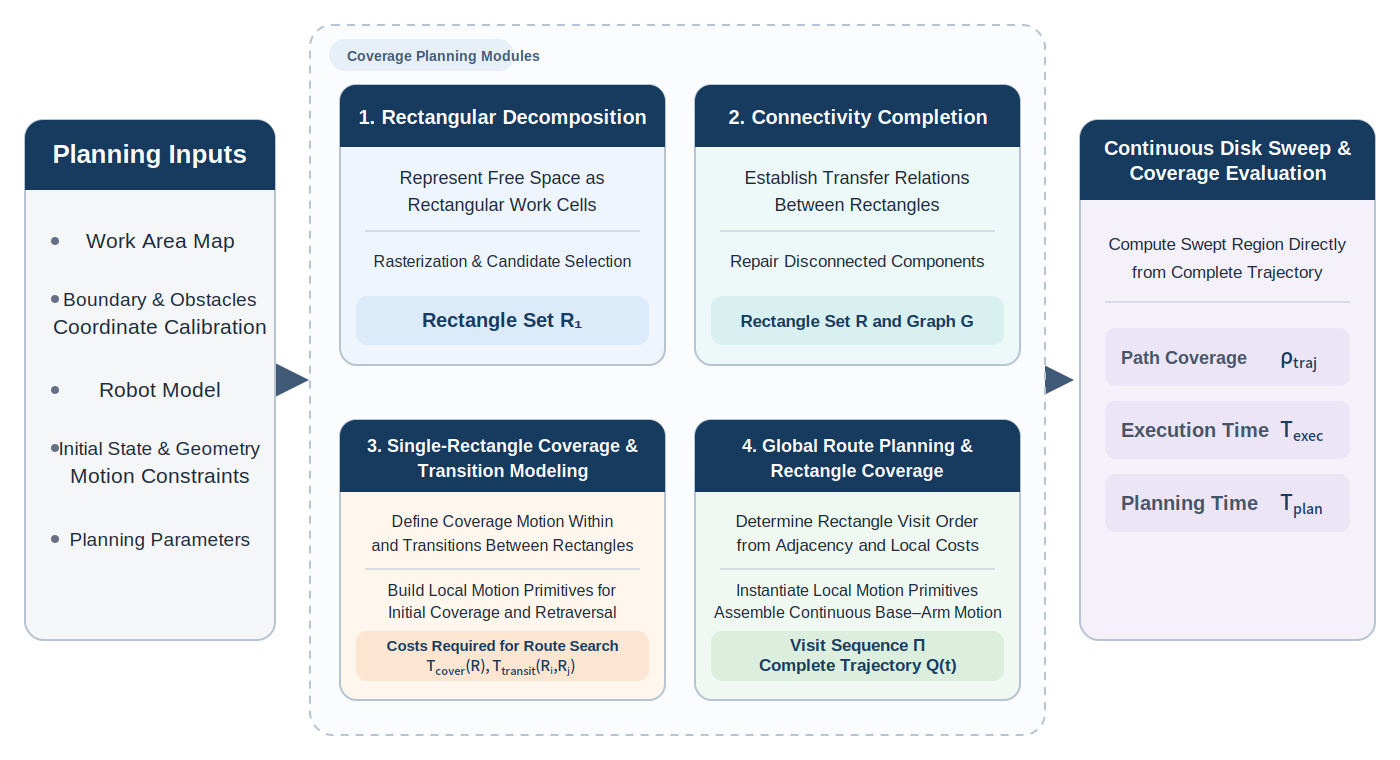
\includegraphics[width=0.98\linewidth]{pipeline_overall_improved_en.png}
  \caption{Coverage-planning framework and principal data flow. The inputs on the left are the work map, coordinate calibration, robot model, initial state, and planning parameters. The four central modules successively produce an initial rectangle set $\mathcal R_1$, a final rectangle set $\mathcal R$ with adjacency graph $G$, entry- and exit-constrained local motion primitives with time costs, and a visitation sequence $\Pi$ with complete trajectory $q(t)$. Continuous disc sweeping then yields coverage ratios, execution time, and planning time.}
  \label{fig:pipeline}
\end{figure}

The rectangular-decomposition module first generates candidate rectangles on a conservative planning grid and selects suitable work units according to newly covered area, rectangle count, and overlap, producing the initial set $\mathcal R_1$. The connectivity-completion module creates geometric adjacency candidates, removes relationships that fail a base--arm transfer check, and inserts bridging rectangles when needed. Its output is a final rectangle set $\mathcal R$ and feasible adjacency graph $G$. An edge in $G$ therefore means not only that two rectangles touch geometrically, but also that at least one local transfer satisfies the geometric and velocity constraints in Eqs.~\eqref{eq:geometric-feasibility} and \eqref{eq:velocity-limits}.

For every rectangle, the local-modeling module constructs two primitive types. A first visit uses a coverage primitive, whereas a repeated visit uses a transit primitive. Their durations depend on the entry and exit states and are denoted by $T_{\mathrm{cover}}(R;q^{\mathrm{in}},q^{\mathrm{out}})$ and $T_{\mathrm{transit}}(R;q^{\mathrm{in}},q^{\mathrm{out}})$, respectively. These costs, together with the transfer costs on graph edges, enter the global route search. After the visitation sequence $\Pi$ has been selected, the same primitives are instantiated as first-visit or repeated-visit motions and concatenated into the complete trajectory. The local motion model thus supports both visitation ordering and final trajectory generation.

Starting from $q_0$, the global module generates a sequence on $G$ that permits repeated transit visits and connects adjacent primitive endpoints, yielding a continuous trajectory $q(t)$ with timing and work-state labels. The evaluation module recovers the disc-center path from $q(t)$ and computes effective-work coverage $\rho_{\mathrm{work}}$, full-trajectory coverage $\rho_{\mathrm{traj}}$, and execution time $T_{\mathrm{exec}}$. The wall-clock time from conservative-grid generation through trajectory evaluation is $T_{\mathrm{plan}}$. The following subsections define the inputs, states, and metrics, then describe each module and the continuous swept-area evaluation.

\subsection{Problem Formulation and Notation}
\label{sec:formulation}

\subsubsection{From a Construction Scene to Planning Inputs}

The required scene information is first extracted from a CAD/BIM model, site-survey data, or localization and mapping output. For a floor to be troweled, a world-coordinate plane $\mathcal F_W$ coincident with the work surface is selected, and the boundary of the current task is specified in that plane. Walls, columns, equipment foundations, embedded components, reserved openings, and areas outside the work boundary are marked as unavailable. The remaining floor inside the boundary on which the disc may operate becomes the target work region. To account for localization error, map error, or additional clearance, unavailable-region contours can be dilated by a margin $\delta_{\mathrm{map}}$ before rasterization. The classified plane is then rasterized and geometrically calibrated to produce a physically scaled binary work map, which is the direct map input to CPP.

Discretization converts heterogeneous geometry from CAD/BIM, field measurement, and mapping into spatial cells at a common resolution. This gives rectangle generation, adjacency testing, collision checking, and coverage calculation a consistent computational basis. At a resolution of $s_p$~m/pixel, the plane becomes a binary map $M$: white pixels are obstacle-free target pixels included in the coverage task, whereas black pixels represent walls, columns, openings, out-of-bound areas, and areas excluded by the safety margin. In result and evaluation images, blue pixels denote portions of the target region already swept by the disc. Blue is an overlay on $M$, not a third input-map class. A rigid transform $T_{WM}$ calibrates image coordinates to world coordinates, so every pixel corresponds to a physical location in metres.

The conversion from planar geometry to the binary map follows uniform labeling and conservative discretization. Regardless of boundary shape, all workable and unavailable regions are projected onto the same plane and classified at one resolution as free or occupied cells. Cells on an obstacle boundary or with ambiguous membership are treated as unavailable to avoid misclassifying obstacle space as workable floor. Straight walls and rectangular foundations map directly to contiguous black cells. Circular columns, curved boundaries, and openings are approximated by staircase boundaries at the selected resolution, optionally enlarged by the safety margin. In regions with irregular boundaries or dense obstacles, the occupancy map preserves the overall shape and connectivity; subsequent rectangle generation, hole filling, and connectivity completion handle them uniformly. The conversion therefore does not require a separate decomposition rule for every geometric shape. Its approximation accuracy is governed jointly by map resolution and safety margin.

\begin{figure}[htbp]
  \centering
  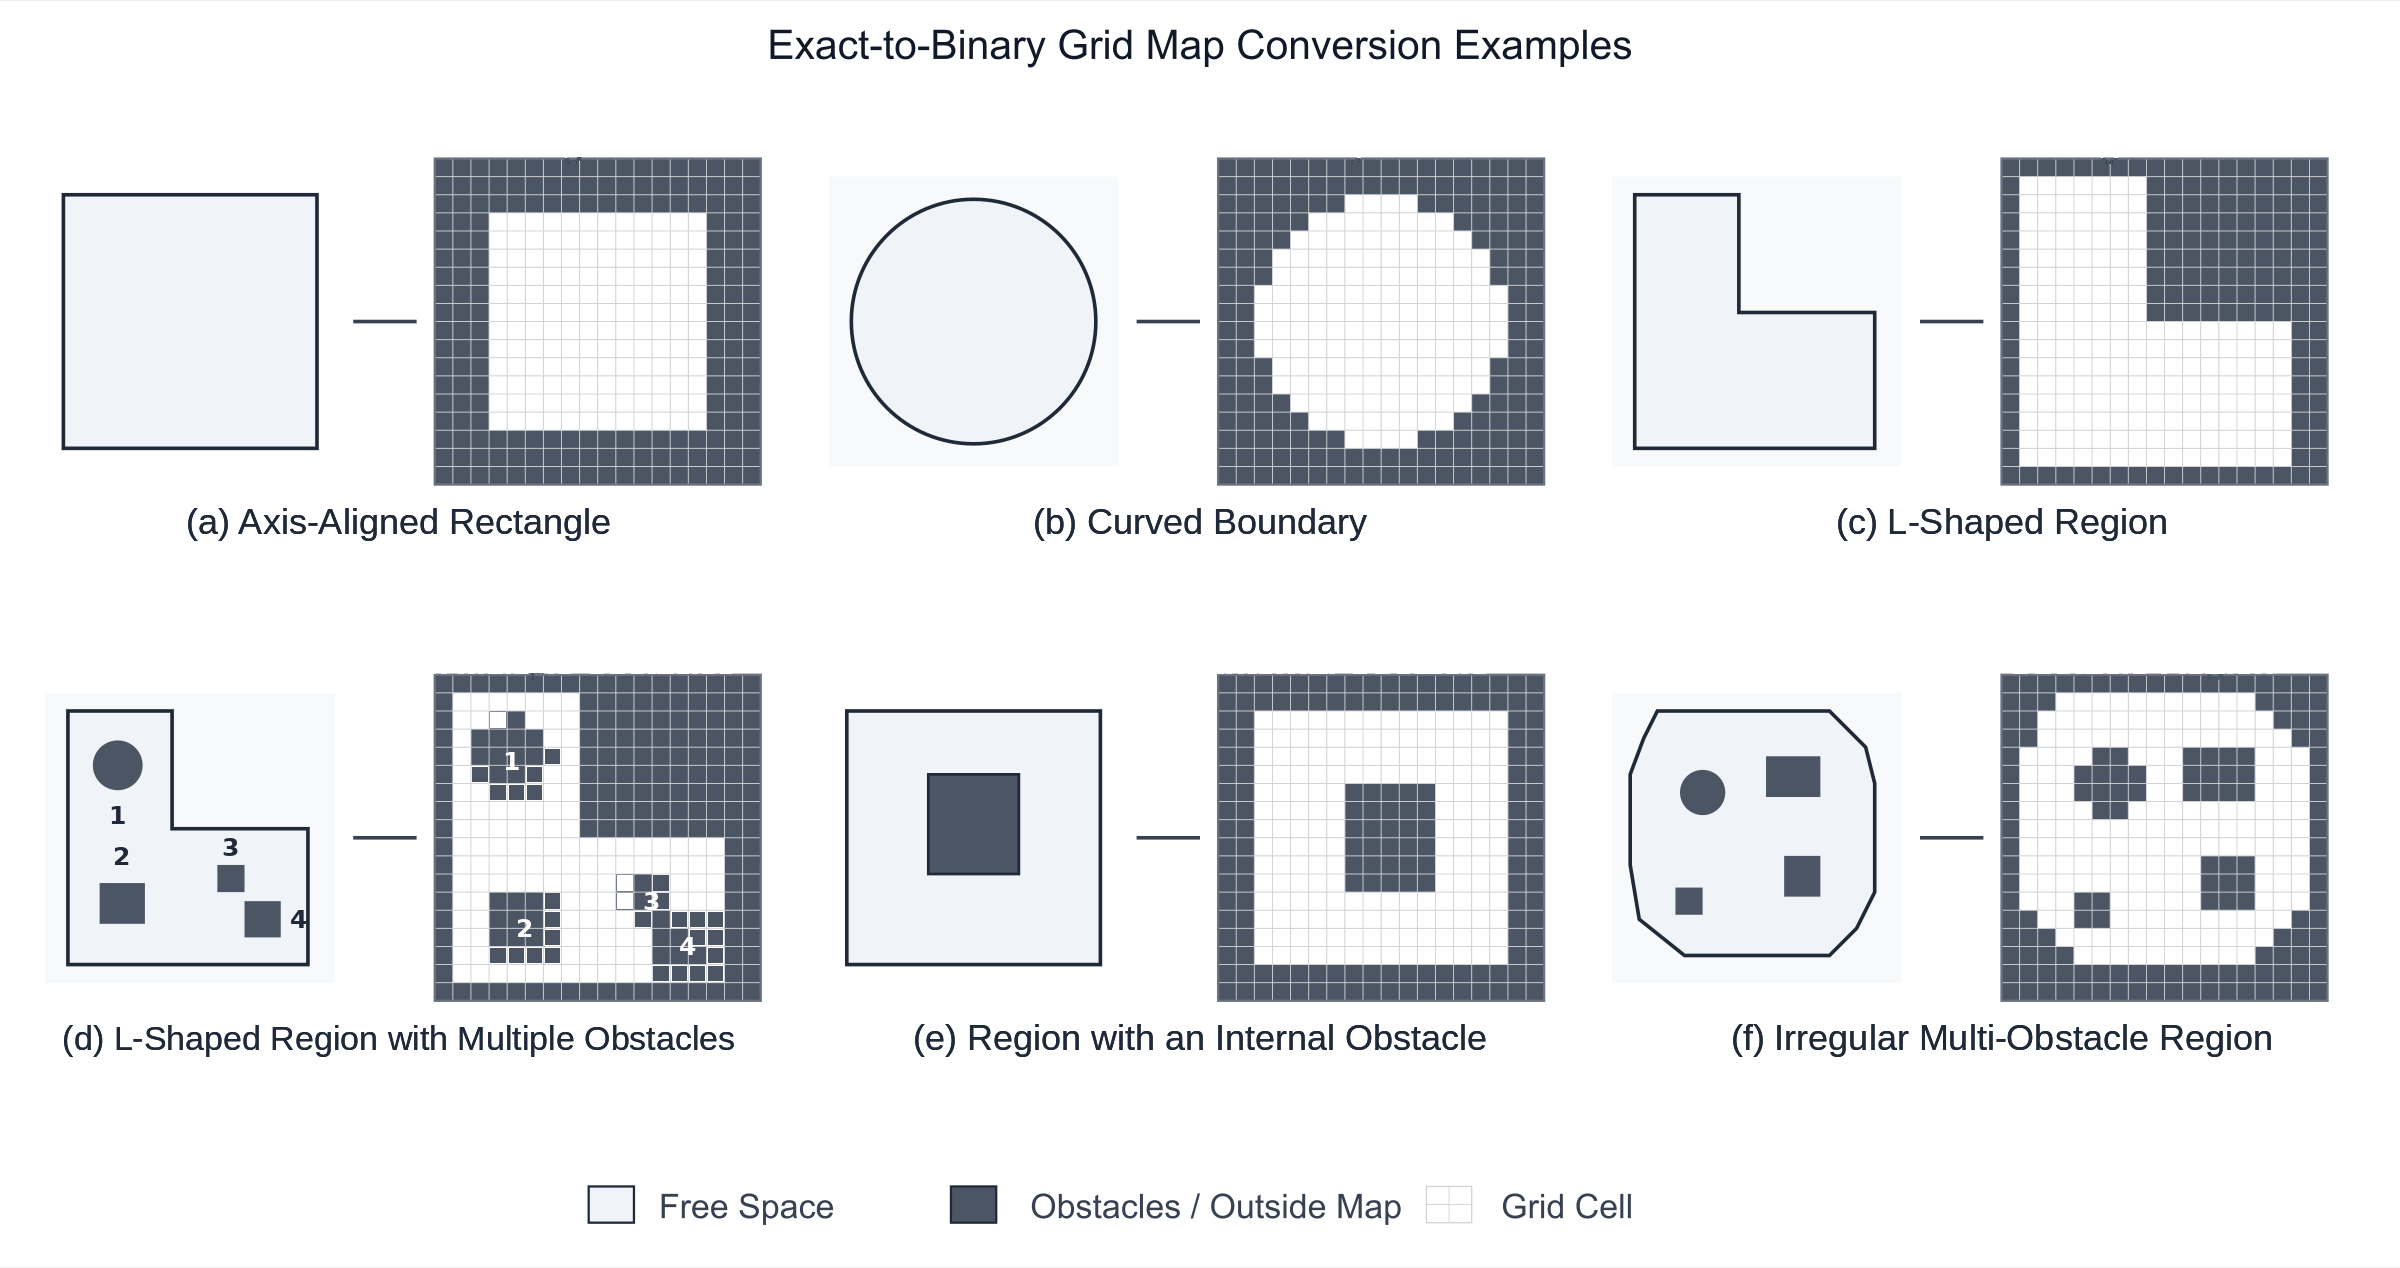
\includegraphics[width=0.96\linewidth]{figure_3_geometric_to_binary_raster.png}
  \caption{Conversion from exact geometric descriptions to the binary raster input. The left column shows exact two-dimensional work regions and rectangular subregions abstracted from CAD/BIM, survey, or mapping data; the right column shows the binary map $M$ used by the planner. White denotes free target area, black denotes obstacles, openings, or out-of-bound regions, and dashed rectangles indicate approximate cells that may support later rectangular candidates. Examples include rectangular rooms, circular or curved boundaries, L-shaped areas, T-junction or corridor connections, regions with columns or openings, and irregular areas with dense obstacles.}
  \label{fig:rasterization-examples}
\end{figure}

After the map has been abstracted, equipment drawings, calibration tests, and controller limits provide the robot model and initial state. The scene input for one planning task is divided into map and robot components:
\begin{equation*}
\mathcal I=\left\langle\mathcal I_{\mathrm{map}},\mathcal I_{\mathrm{robot}}\right\rangle,
\end{equation*}
where
\begin{equation*}
\mathcal I_{\mathrm{map}}=\left\langle M,s_p,T_{WM}\right\rangle.
\end{equation*}
Here $M$ is the $H_p\times W_p$ binary work map generated from CAD/BIM, survey, or mapping data; $s_p$ converts pixel distance and area to metres and square metres; and $T_{WM}$ is the planar rigid transform from the map frame to the world frame, used to convert planned map coordinates into executable site coordinates.

The robot component is
\begin{equation*}
\mathcal I_{\mathrm{robot}}=\left\langle q_0,\Theta_R\right\rangle.
\end{equation*}
The initial base position, heading, and arm angle in $q_0$ are obtained from the site-localization system and arm encoder. The parameter set $\Theta_R$ contains the base length $l_c$ and width $w_c$, arm-link collision radius $r_a$, troweling-disc radius $r_d$ (diameter $2r_d$), arm length $L$, distance $d_p$ from the base center to the arm pivot, arm-angle limits, maximum base linear and angular velocities, and maximum arm angular velocity. Together, these parameters determine occupied geometry, the disc coverage footprint, and trajectory executability.

\begin{figure}[htbp]
  \centering
  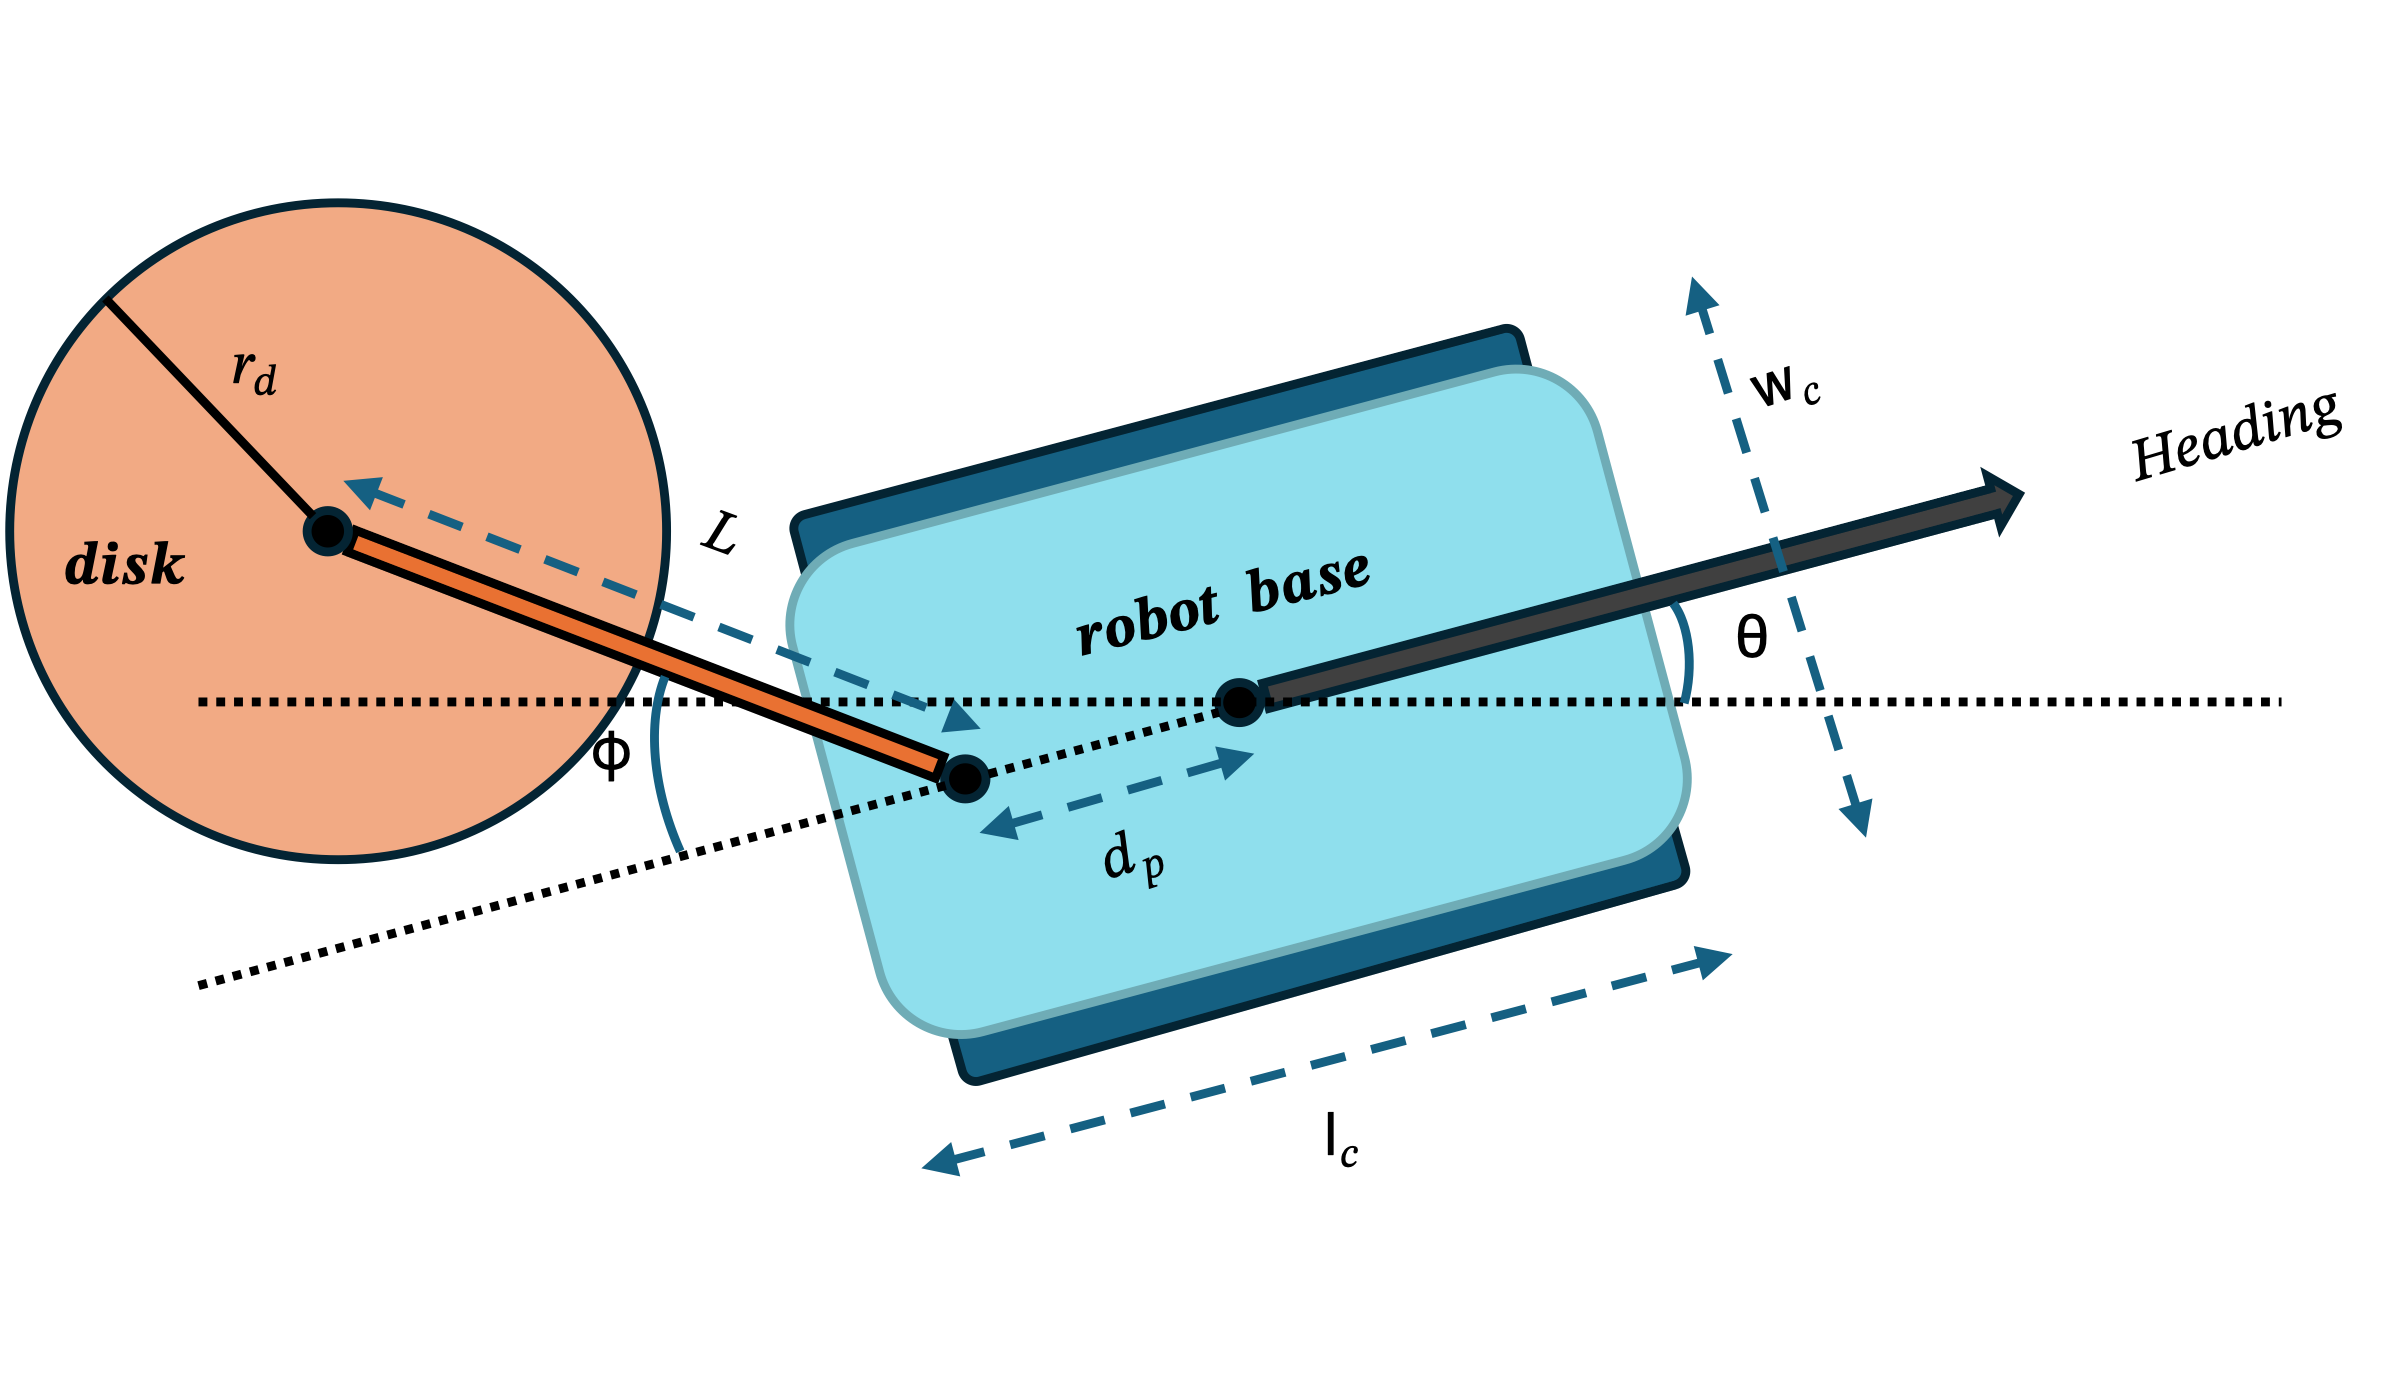
\includegraphics[width=0.82\linewidth]{figure_4_body_arm_disc_model.png}
  \caption{Geometry and motion parameters of the base--arm--disc system. The diagram identifies the base center, heading $\theta$, relative arm angle $\phi$, disc radius $r_d$, arm length $L$, base-center-to-pivot offset $d_p$, and base length and width $l_c,w_c$. These quantities determine the robot's occupied geometry and the disc-center position in Eq.~\eqref{eq:disc-center}.}
  \label{fig:robot-geometry}
\end{figure}

In addition to these scene inputs, the algorithm uses a planning configuration $\Psi_P$: planning-cell size $g$, minimum rectangle side length, candidate-selection parameters $\alpha$ and $\beta$, candidate truncation count, scan and connectivity strategies, and random seed. The configuration controls decomposition and search but is not part of the map or robot model abstracted from the physical scene.

\subsubsection{Planning Model and Notation}

Let the input map be
\begin{equation*}
M\in\{0,255\}^{H_p\times W_p},
\end{equation*}
where $M_{uv}=0$ is an obstacle pixel and $M_{uv}=255$ a free pixel. With physical pixel size $s_p$, the free-pixel set is
\begin{equation*}
\mathcal P_F=\{(u,v)\mid M_{uv}=255\}.
\end{equation*}
All subsequent positions and distances are transformed by $T_{WM}$ into a metric world frame; for clarity, the transform is omitted from the remaining notation.

The robot state is
\begin{equation*}
q(t)=\bigl(x_c(t),y_c(t),\theta(t),\phi(t)\bigr),
\end{equation*}
with state space $\mathcal Q=\mathbb R^2\times S^1\times[\phi_{\min},\phi_{\max}]$. Here $(x_c,y_c)$ is the base center, $\theta$ the base heading, and $\phi$ the arm angle relative to the base. Let $\mathbf p_c=(x_c,y_c)$ and $\mathbf e(\gamma)=(\cos\gamma,\sin\gamma)$. For arm length $L$ and base-center-to-pivot offset $d_p$, the center of the circular disc is
\begin{equation}
\mathbf p_d(q)=\mathbf p_c-d_p\mathbf e(\theta)+L\mathbf e(\theta+\pi+\phi).
\tag{1}
\label{eq:disc-center}
\end{equation}
Equation~\eqref{eq:disc-center} is the sum of two translations: from the base center to the arm pivot and from the pivot to the disc center. As shown in Fig.~\ref{fig:robot-geometry}, $\mathbf e(\theta)$ points along the base heading, and the pivot lies $d_p$ behind the base center, so
\begin{equation*}
\mathbf p_p=\mathbf p_c-d_p\mathbf e(\theta).
\end{equation*}
The arm angle $\phi$ is defined as the signed rotation from the rearward base axis, positive counterclockwise. Since the rearward axis is rotated by $\pi$ from the forward heading, the pivot-to-disc direction is $\theta+\pi+\phi$, and its displacement is $L\mathbf e(\theta+\pi+\phi)$. For example, when $\theta=0$ and $\phi=0$, the base faces the positive world $x$-axis, the pivot is at $(x_c-d_p,y_c)$, and the disc center is at $(x_c-d_p-L,y_c)$: the arm extends directly behind the base. Changing $\theta$ rotates the pivot and arm with the base; changing $\phi$ at fixed $\theta$ moves the disc center along a radius-$L$ arc about the pivot.

For disc radius $r_d$, the instantaneous work region at one pose is
\begin{equation}
\mathcal D(q)=\{\mathbf z\in\mathbb R^2\mid\|\mathbf z-\mathbf p_d(q)\|_2\le r_d\}.
\tag{2}
\label{eq:instantaneous-disc}
\end{equation}
The region swept by a continuous trajectory $q:[0,T]\rightarrow\mathcal Q$ is
\begin{equation}
\mathcal C(q)=\bigcup_{t\in[0,T]}\mathcal D(q(t)).
\tag{3}
\label{eq:swept-area}
\end{equation}

To distinguish disc reachability from whole-robot feasibility, let $\mathcal O_M$ be the unavailable region corresponding to black pixels in world coordinates, $\mathcal B(q)$ the rotated $l_c\times w_c$ base rectangle, and $\mathcal A(q)$ a capsule of radius $r_a$ around the arm link. A state is geometrically feasible only if
\begin{equation}
\bigl(\mathcal B(q)\cup\mathcal A(q)\cup\mathcal D(q)\bigr)\cap\mathcal O_M=\varnothing.
\tag{3a}
\label{eq:geometric-feasibility}
\end{equation}
All feasible states form $\mathcal Q_F\subseteq\mathcal Q$. For a motion segment $q_s:[0,T_s]\rightarrow\mathcal Q$, the method requires $q_s(t)\in\mathcal Q_F$ for every $t\in[0,T_s]$ and
\begin{equation}
|v(t)|\le v_{\max},\qquad
|\dot\theta(t)|\le\omega_{\max},\qquad
|\dot\phi(t)|\le\omega_{a,\max}.
\tag{3b}
\label{eq:velocity-limits}
\end{equation}
Straight motion, in-place rotation, arm adjustment, and other primitives are adaptively subdivided, and Eq.~\eqref{eq:geometric-feasibility} is checked over every subinterval. Consequently, later rectangle adjacencies and entry states are candidates only; a transfer enters the final planning graph only after passing this check.

Under Eqs.~\eqref{eq:geometric-feasibility} and \eqref{eq:velocity-limits}, the algorithm is assessed at three levels: work quality, trajectory-execution efficiency, and planning efficiency. The corresponding objectives are
\begin{equation}
\max \rho_{\mathrm{work}}(q),\qquad
\min T_{\mathrm{exec}}(q),\qquad
\min T_{\mathrm{plan}}.
\tag{4}
\label{eq:objectives}
\end{equation}
The effective-work coverage ratio $\rho_{\mathrm{work}}(q)$ is the fraction of the target area swept by the disc during work-labeled segments. The nominal execution time $T_{\mathrm{exec}}(q)$ runs from the initial state to completion and includes the initial connection, effective work, turns, arm adjustments, and inter-region transfers. The wall-clock planning time $T_{\mathrm{plan}}$ covers the algorithm from conservative-grid generation through trajectory assembly and coverage evaluation.

These measures play distinct roles. The task-level quality measure $\rho_{\mathrm{work}}$ is encouraged indirectly through free-space rectangle representation, rewards for new coverage, and overlap penalties, then computed from the continuous disc sweep in Eqs.~\eqref{eq:disc-center}--\eqref{eq:swept-area} after the complete trajectory is available. The route-level objective $T_{\mathrm{exec}}$ supplies time costs to local primitives and global visitation candidates; the algorithm selects feasible trajectories with low proxy cost but does not claim a global minimum. The planning-time measure $T_{\mathrm{plan}}$ is not a decision variable of $q$; it is a design objective controlled by hierarchical decomposition, polynomial-time heuristics, and candidate truncation. This separation motivates the hierarchical heuristic framework.

\subsection{Conservative Rasterization and Rectangular Decomposition}

The decomposition module first converts the pixel map into a coarser planning grid. Let each square planning cell contain $g\times g$ pixels, and let $\Omega_{ij}$ be the pixel block associated with planning cell $(i,j)$. Conservative rasterization gives
\begin{equation}
B_{ij}=\begin{cases}
1, & \text{if } M_{uv}=255,\quad \forall (u,v)\in\Omega_{ij},\\
0, & \text{otherwise}.
\end{cases}
\tag{5}
\label{eq:conservative-raster}
\end{equation}
Thus, $B_{ij}=1$ means that the planning cell can support rectangle generation; $B_{ij}=0$ means that it contains or touches an obstacle. The rule sacrifices some free area near obstacles but guarantees that subsequent rectangular candidates do not cross known obstacles.

On $B$, the algorithm scans maximal contiguous runs of free cells by rows and by columns, extending them across adjacent scan lines as long as every enclosed cell remains free. This produces axis-aligned candidates of the form
\begin{equation}
R=[x_1,x_2]\times[y_1,y_2],
\tag{6}
\label{eq:rectangle}
\end{equation}
with all planning cells inside $R$ free. Candidates whose width or height is below a specified minimum are removed. The remainder are ordered first by decreasing area and, for equal areas, by increasing row and column coordinates of the upper-left and then lower-right corner. Only the first $C_{\max}$ candidates from each scan direction are retained. This deterministic truncation controls rapid growth in candidate count while making the candidate set repeatable for fixed inputs and parameters.

Candidate selection is formulated as a penalized maximum-coverage problem. Let $\mathcal U(R)$ be the set of planning cells covered by $R$ and $\mathcal A$ the cells already covered by selected rectangles. The marginal utility of selecting $R$ is
\begin{equation}
\Delta(R\mid\mathcal A)=|\mathcal U(R)\setminus\mathcal A|-\alpha-\beta|\mathcal U(R)\cap\mathcal A|.
\tag{7}
\label{eq:marginal-utility}
\end{equation}
Cardinalities are measured in planning cells, so $\alpha$ has units of cells and $\beta$ is dimensionless. The first term rewards new coverage; the other terms penalize rectangle count and overlap. The algorithm repeatedly selects the row-scan candidate with the largest positive marginal utility, using the deterministic ordering above to break ties. It then processes the column-scan pool relative to the current $\mathcal A$, so column-oriented rectangles mainly supplement vertical structures poorly represented by row scans. The two greedy stages produce the initial selection.

Candidate truncation or the penalties may leave a small number of free cells uncovered. A deterministic hole-filling stage therefore selects the first uncovered free cell in row-major order as a seed, enumerates maximal axis-aligned obstacle-free rectangles containing the seed, and selects the largest. Remaining ties are resolved by rectangle width and upper-left coordinates. The selected rectangle is added and $\mathcal A$ updated until every usable planning cell belongs to at least one rectangle. The resulting set, before connectivity repair, is $\mathcal R_1$. Minimum side length, $C_{\max}$, $\alpha$, $\beta$, and scan direction are included in $\Psi_P$.

\subsection{Connectivity Completion and Final Segmentation}

Covering every free planning cell with rectangles does not ensure that the robot can move continuously between them. The method therefore constructs an undirected graph
\begin{equation}
G=(V,E),
\tag{8}
\label{eq:feasible-graph}
\end{equation}
over $\mathcal R_1$, with node $v_i\in V$ representing rectangle $R_i$. Shared boundaries, contact, and overlap generate geometric adjacency candidates only. For each candidate pair $(R_i,R_j)$, a finite set of handoff poses is generated in the intersection or along the closest opposing boundaries. The algorithm then attempts to connect an exit state of the first rectangle to an entry state of the second. Edge $(v_i,v_j)$ is added only if at least one transfer primitive satisfies Eqs.~\eqref{eq:geometric-feasibility} and \eqref{eq:velocity-limits}. The edge stores the minimum time proxy $c_{ij}$ among all feasible handoffs. Graph $G$ consequently represents executable robot transfers, not merely geometric contact between rectangles.

If $G$ has multiple connected components, the algorithm searches the unselected candidates for bridging rectangles. A candidate $R_b$ is a bridge if, after insertion, it forms feasible edges with rectangles in at least two previously distinct components. Preference is given to rectangles with little new area and low feasible-transfer cost:
\begin{equation}
R_b^\star=\arg\min_{R_b\in\mathcal B}\left(|\mathcal U(R_b)\setminus\mathcal A|+\lambda_b\sum c_{ib}\right),
\tag{9}
\label{eq:bridge-cost}
\end{equation}
where $\mathcal B$ is the current bridge-candidate set, the sum contains only edges used to connect components, and $\lambda_b$ weights transfer time. Relevant edges and connected components are recomputed after every insertion, until $G$ becomes connected. If $\mathcal B$ is empty while $G$ remains disconnected, no single continuous coverage trajectory is supported by the current candidate set and parameters. The method reports connectivity failure and does not proceed to global route planning.

\begin{algorithm}[htbp]
\caption{Rectangle segmentation and connectivity completion}
\label{alg:segmentation}
\small
\begin{algorithmic}[1]
\Require Conservative free-cell grid $B$, planning parameters $\Psi_P$, robot model $\Theta_R$
\Ensure Rectangle set $\mathcal R$ and feasible graph $G$, or connectivity failure
\State $F\gets\{u:B(u)=1\}$; $\mathcal R\gets\varnothing$; $\mathcal A\gets\varnothing$
\State $(C_r,C_c)\gets\mathrm{ScanAndTruncate}(B,\Psi_P)$
\State $C_{\mathrm{all}}\gets C_r\cup C_c$
\For{$C\in(C_r,C_c)$, in this order}
  \While{$\exists R\in C:\Delta(R\mid\mathcal A)>0$}
    \State $R^\star\gets\arg\max_{R\in C}\Delta(R\mid\mathcal A)$ \Comment{Eq.~\eqref{eq:marginal-utility}; deterministic ties}
    \State $\mathcal R\gets\mathcal R\cup\{R^\star\}$; $\mathcal A\gets\mathcal A\cup\mathcal U(R^\star)$
    \State $C\gets C\setminus\{R^\star\}$
  \EndWhile
\EndFor
\While{$\mathcal A\neq F$}
  \State $u\gets\mathrm{FirstUncovered}(F\setminus\mathcal A)$
  \State $R^\star\gets\mathrm{LargestMaximalRectangle}(B,u)$ \Comment{deterministic ties}
  \State $\mathcal R\gets\mathcal R\cup\{R^\star\}$; $\mathcal A\gets\mathcal A\cup\mathcal U(R^\star)$
\EndWhile
\State $\mathcal R_1\gets\mathcal R$; $G\gets\mathrm{FeasibleGraph}(\mathcal R_1,\Theta_R)$
\While{$G$ is disconnected}
  \State $\mathcal B\gets\mathrm{FeasibleBridges}(C_{\mathrm{all}}\setminus\mathcal R,G,\Theta_R)$
  \If{$\mathcal B=\varnothing$}
    \State \Return connectivity failure
  \EndIf
  \State $R_b^\star\gets\mathrm{MinBridgeCost}(\mathcal B)$ \Comment{Eq.~\eqref{eq:bridge-cost}}
  \State $\mathcal R\gets\mathcal R\cup\{R_b^\star\}$; $G\gets\mathrm{UpdateFeasibleGraph}(G,R_b^\star)$
\EndWhile
\State \Return $(\mathcal R,G)$
\end{algorithmic}
\end{algorithm}

Algorithm~\ref{alg:segmentation} summarizes the complete process from conservative rasterization to the final graph. The overlap penalty in Eq.~\eqref{eq:marginal-utility} suppresses redundant rectangles within a candidate pool; hole filling represents every free planning cell; and bridging adds rectangles only when the current set cannot form a connected feasible graph. ``Connected'' always refers to graph connectivity after complete robot-transfer checks, not merely topological connectivity of free cells or the geometric rectangle union.

Let the planning grid be $H\times W$, the truncated candidate count $C$, the final rectangle count $n$, and the mean candidate area $A$ cells. Candidate generation has worst-case complexity $O(HW(H+W))$. With a naive set implementation, greedy selection is approximately $O(CnA)$. Adjacency-candidate enumeration is $O(n^2)$, with a finite number of local-motion checks per edge. The minimum side length, candidate truncation, and deterministic ordering jointly limit practical problem size. Since later graph search and local-primitive instantiation grow with $n$, controlling the rectangle count during decomposition directly affects $T_{\mathrm{plan}}$.

\subsection{Single-Rectangle Coverage Primitive}

The rectangle-coverage module supplies the local motion primitive. Given a rectangle $R$, feasible entry pose $q^{\mathrm{in}}$, feasible exit pose $q^{\mathrm{out}}$, and robot parameters, it generates a continuous motion segment. On the first occurrence of $R$ in the global sequence, the robot executes the back-and-forth coverage shown in Fig.~\ref{fig:rectangle-primitive}; if $R$ has already been covered, only an entry-to-exit transit motion is generated. Both primitive types retain the complete robot state, duration, and work-state label.

\begin{figure}[htbp]
  \centering
  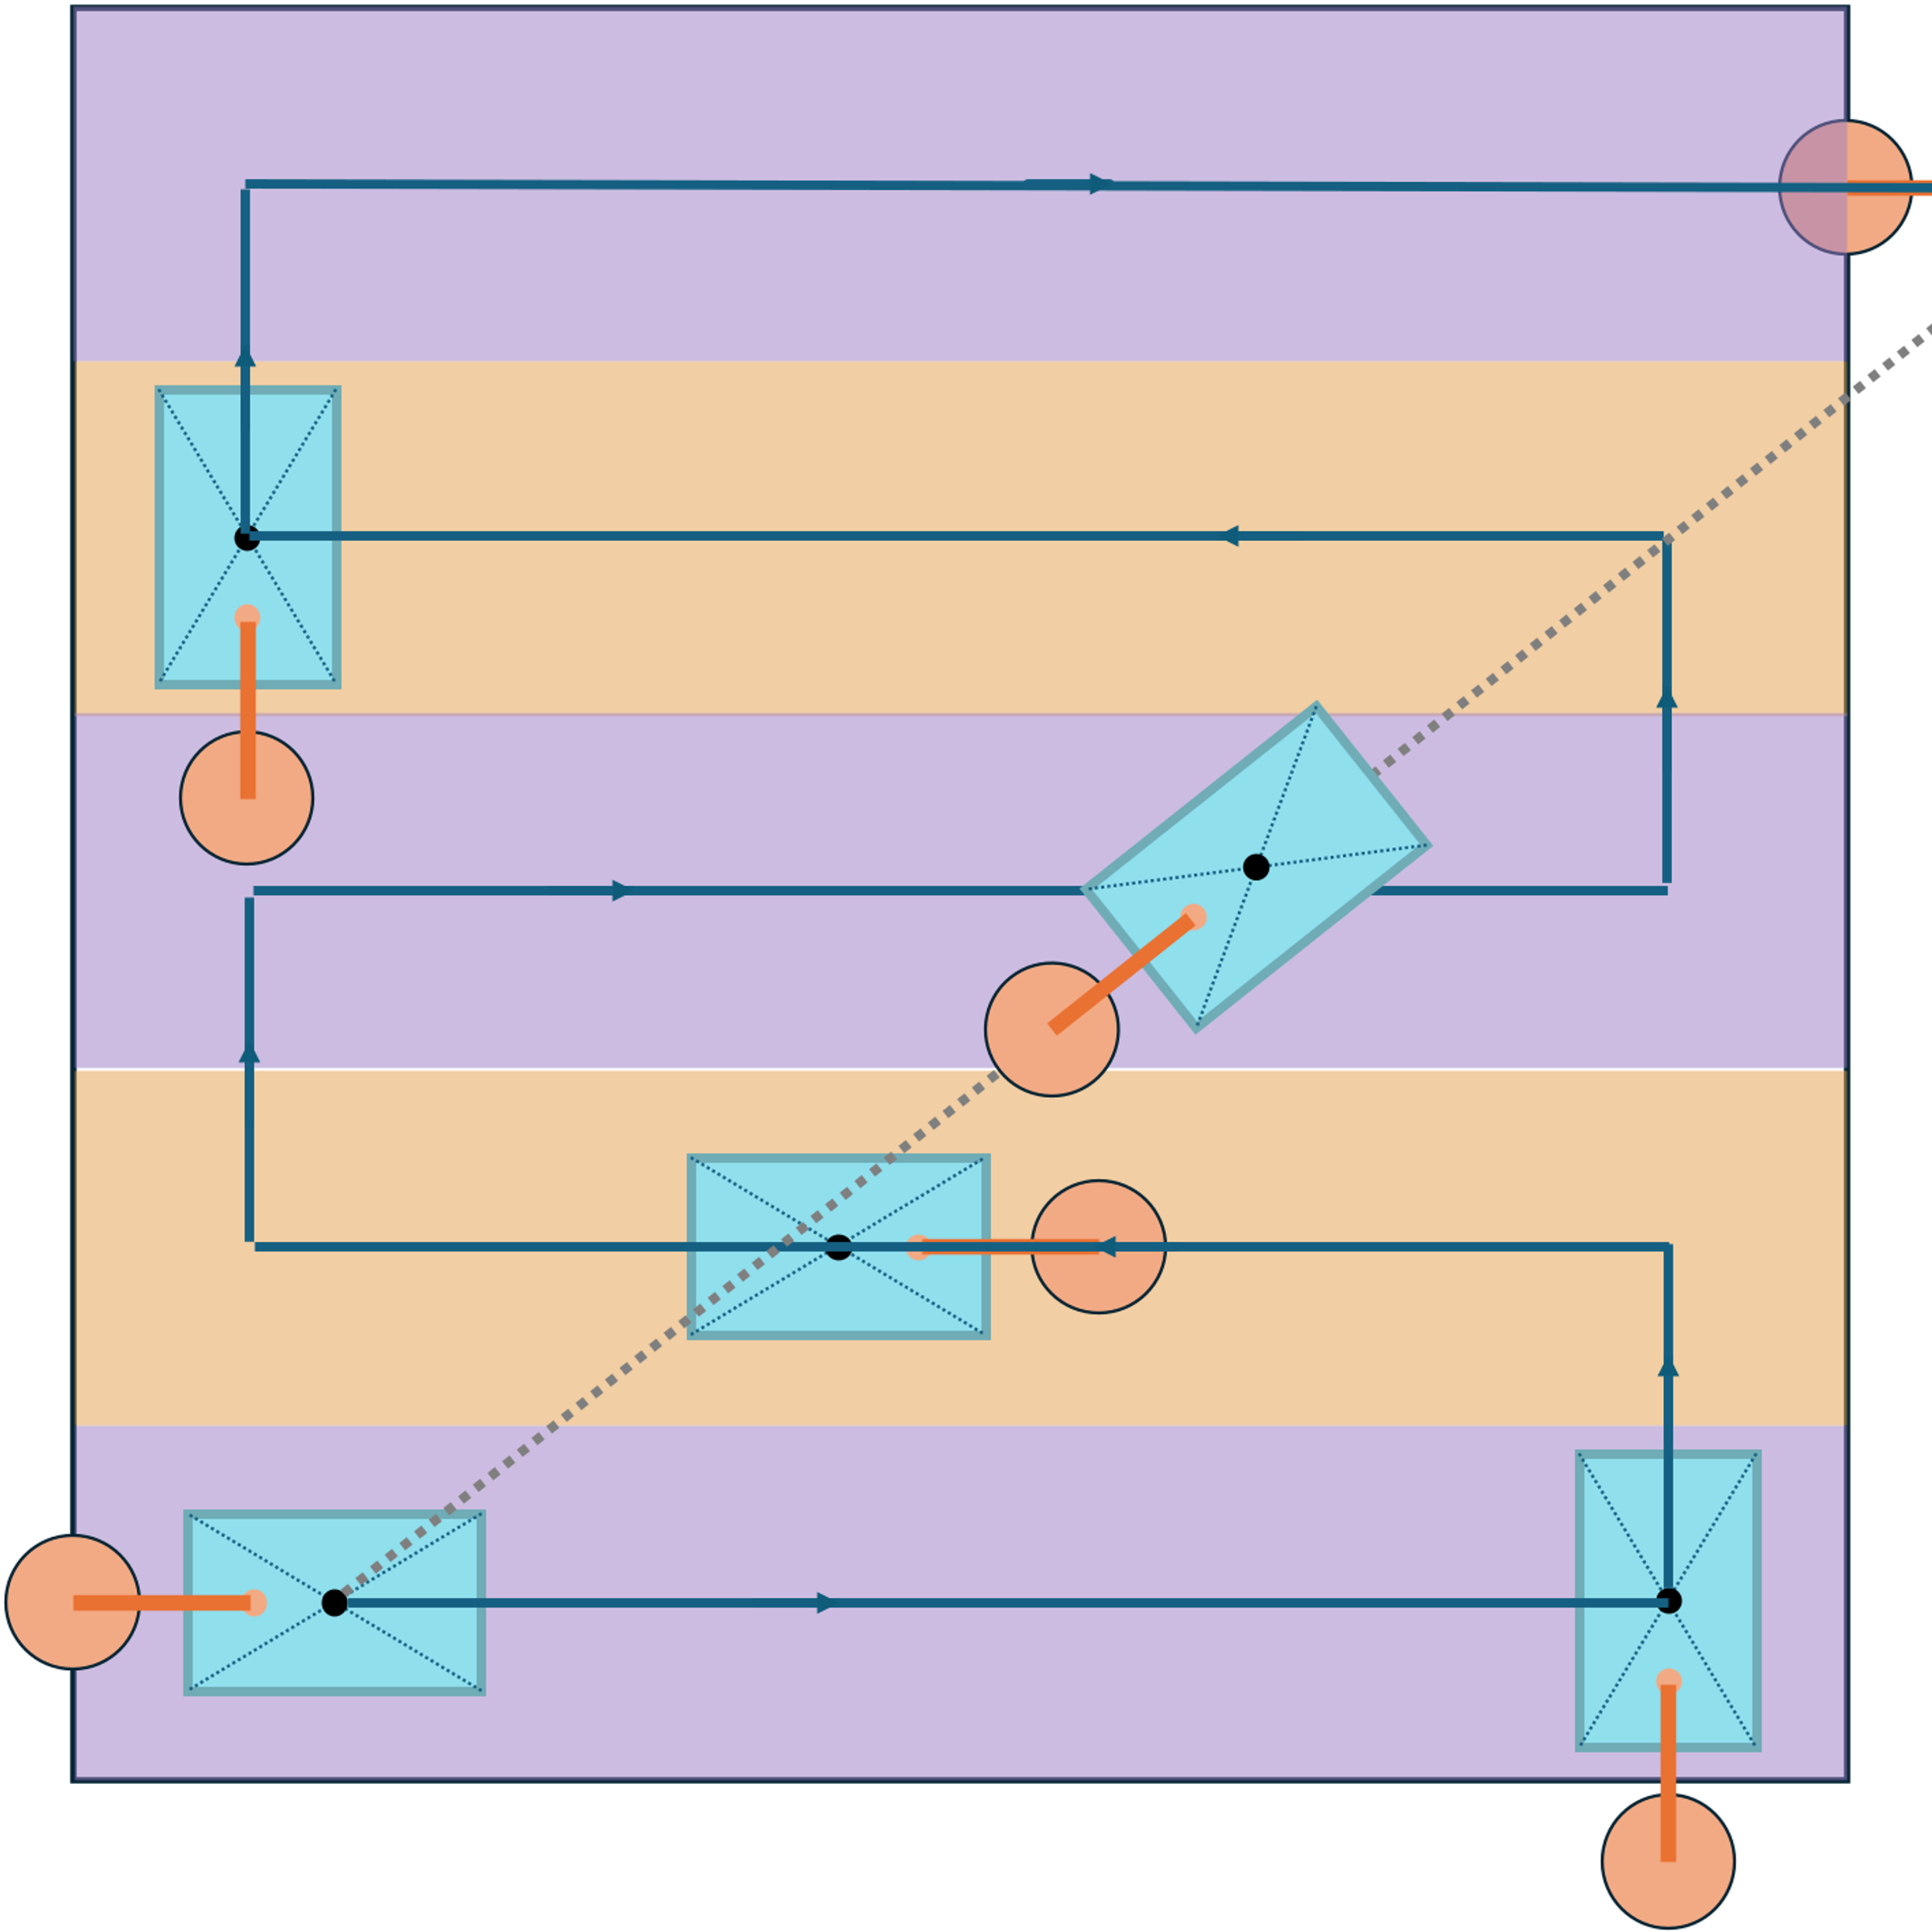
\includegraphics[width=0.84\linewidth]{figure_6_single_rectangle_coverage.png}
  \caption{Single-rectangle coverage primitive. The disc entry and exit are determined by neighboring rectangles or the initial state. The local planner compares time proxies for both sweep directions and feasible starting corners, then covers the rectangle through forward base motion and reciprocal arm swinging.}
  \label{fig:rectangle-primitive}
\end{figure}

\subsubsection{Entry and Exit Poses}

Entry and exit candidates are jointly determined by the predecessor and successor of a rectangle in the visitation sequence. If $R_i$ is followed by $R_j$, a finite set of disc handoff points is sampled uniformly in their shared region or along their opposing boundaries. An entry to the first rectangle must also be reachable from $q_0$, and an exit from the final rectangle is selected among its remaining feasible boundary candidates. Each candidate specifies the disc center, base heading, and reference arm angle rather than only a boundary point.

For disc points on the left, right, lower, and upper boundaries, the nominal headings are $\pi$, $0$, $3\pi/2$, and $\pi/2$, respectively, so that the base in its retracted configuration lies outside the corresponding rectangle boundary. This rule generates nominal candidates only. Near dense obstacles or narrow boundaries, the externally positioned base may still enter unavailable space and therefore cannot be accepted without checking.

Given a boundary pose $(\mathbf p_d,\theta)$ for the disc center, the base center in the retracted reference configuration is recovered as
\begin{equation}
\mathbf p_c=\mathbf p_d+(d_p+L)\mathbf e(\theta).
\tag{10}
\label{eq:entry-base-center}
\end{equation}
The state and its connection from the preceding primitive are then checked against Eqs.~\eqref{eq:geometric-feasibility} and \eqref{eq:velocity-limits}. If a check fails, the handoff point is moved along the same boundary, followed by trials on an adjacent boundary and with the alternative heading. Only candidates with a feasible complete connection enter the local cost comparison. If a visit admits no feasible entry--exit pair, the corresponding global sequence cannot be instantiated.

\subsubsection{Starting Corner, Strip Width, and Swing Amplitude}

\begin{figure}[htbp]
  \centering
  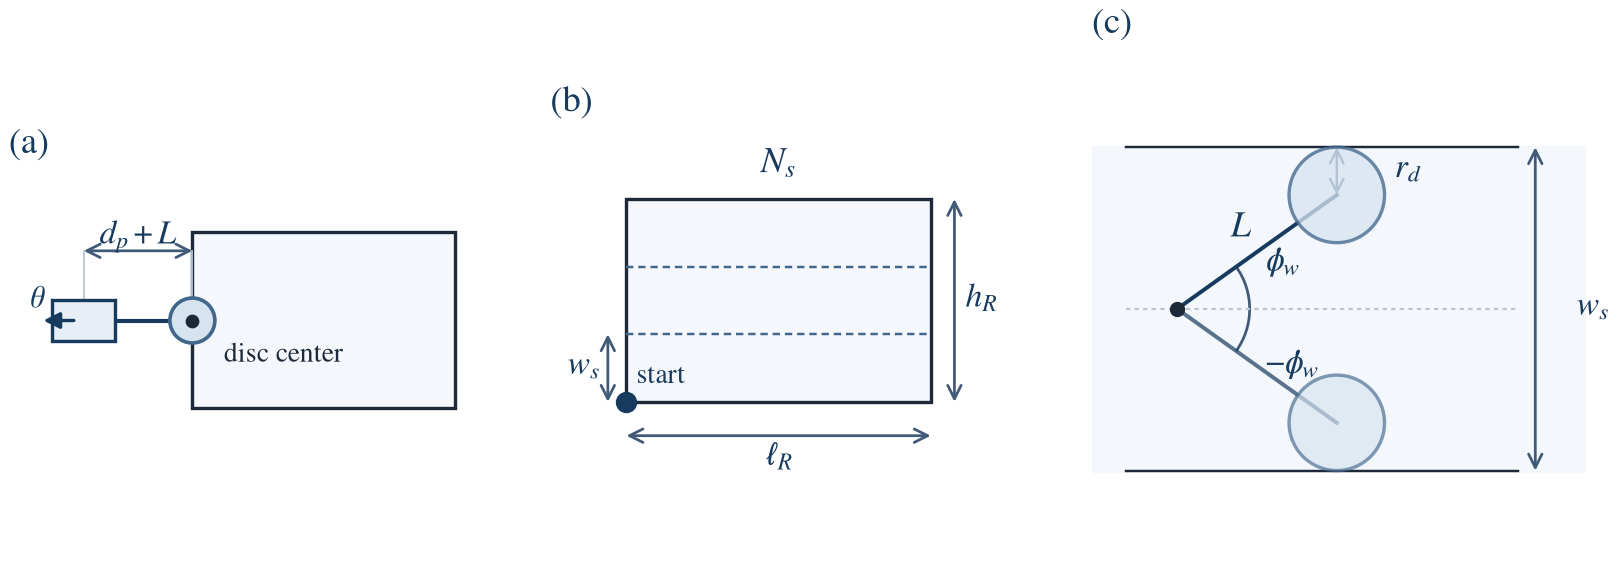
\includegraphics[width=0.92\linewidth]{figure_strip_geometry.png}
\end{figure}

Let $\ell_R$ and $h_R$ be the rectangle dimensions parallel and perpendicular to the work strips. The local planner uses the longer axis by default to reduce lane changes, but also generates a solution along the other axis. Across the two sweep directions and their feasible starting corners, it compares the total time proxy for entry connection, coverage, lane changes, and exit connection. Thus $h_R$ always denotes the transverse extent crossed collectively by the strips, whereas $\ell_R$ is the travel length of one strip.

For each sweep direction, the planner filters the four corners to retain starting points reachable from the entry and connectable to the exit; the parity of the strip count determines the coverage endpoint. It selects the feasible combination with the minimum sum of non-working motion and local coverage time. Entry, sweep direction, starting corner, strip-count parity, and exit therefore jointly determine the primitive; the start is not chosen merely as the nearest corner in Euclidean distance.

Coverage inside the rectangle follows a Boustrophedon pattern, but the work width is not fixed. It is determined by the maximum usable arm angle and disc radius. For arm limits $[\phi_{\min},\phi_{\max}]$, the symmetric usable angle is
\begin{equation}
\phi_s=\min\{|\phi_{\min}|,|\phi_{\max}|,\pi/2\}.
\tag{11}
\label{eq:symmetric-angle}
\end{equation}
Over one full left--right swing, the lateral width approximately reachable by the disc-center path, including disc radius, is
\begin{equation}
w_{\max}=2(L\sin\phi_s+r_d).
\tag{12}
\label{eq:max-width}
\end{equation}
For transverse rectangle dimension $h_R$, the required number of strips and actual strip width are
\begin{equation}
N_s=\left\lceil\frac{h_R}{w_{\max}}\right\rceil,
\qquad
w_s=\frac{h_R}{N_s}.
\tag{13}
\label{eq:strip-count}
\end{equation}
The half-amplitude required to cover a strip of width $w_s$ is
\begin{equation}
\phi_w=\begin{cases}
0, & w_s\le 2r_d,\\
\arcsin\!\left(\dfrac{w_s/2-r_d}{L}\right), & w_s>2r_d,
\end{cases}
\tag{14}
\label{eq:swing-amplitude}
\end{equation}
clipped to $[0,\phi_s]$. This prevents systematic gaps between adjacent strips due to insufficient swing amplitude.

\subsubsection{Coupling Between Base and Arm Speeds}

\begin{figure}[htbp]
  \centering
  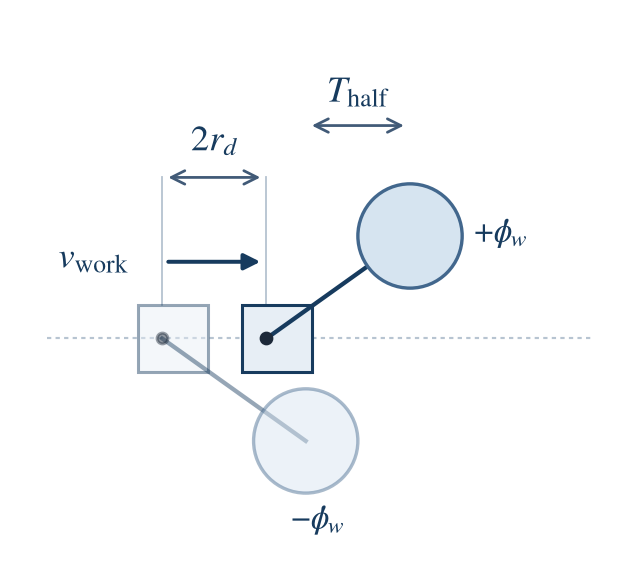
\includegraphics[width=0.78\linewidth]{figure_speed_coupling.png}
\end{figure}

Each strip combines straight base motion with periodic arm swinging. Let the maximum arm angular velocity be $\omega_{a,\max}$ and maximum base linear velocity $v_{\max}$. The time for the arm to move from $-\phi_w$ to $+\phi_w$ is
\begin{equation}
T_{\mathrm{half}}=\frac{2\phi_w}{\omega_{a,\max}}.
\tag{15}
\label{eq:half-cycle}
\end{equation}
The base work speed cannot be chosen from the mechanical limit alone if consecutive half-sweeps are to overlap sufficiently in the direction of travel. The method uses the following heuristic upper bound. If $\phi_w=0$, let $v_{\mathrm{safe}}=+\infty$; otherwise,
\begin{equation}
v_{\mathrm{safe}}=\frac{2r_d}{T_{\mathrm{half}}}.
\tag{16}
\label{eq:safe-speed}
\end{equation}
The work speed is
\begin{equation}
v_{\mathrm{work}}=\min(v_{\max},v_{\mathrm{safe}}).
\tag{17}
\label{eq:work-speed}
\end{equation}
When the arm is slow or the amplitude large, Eq.~\eqref{eq:work-speed} reduces the base speed so that the forward distance between adjacent half-sweeps does not exceed the disc diameter. This is a conservative rule derived from local sweep spacing, not a proof of complete coverage for every continuous arm trajectory. The actual swept area is therefore still checked after local motion generation by the procedure in Section~\ref{sec:coverage-evaluation}. The same relationship underlies the later experimental analysis of the arm-to-base speed ratio.

\subsubsection{Time Model for First and Repeated Visits}

The first visit to a rectangle includes motion to the starting corner, coverage of all strips, lane changes, turns, arm deployment and retraction, and departure from the rectangle. If strip $k$ has length $\ell_k$, lane-change segment $k$ has length $d_k$, base rotation $m$ is $\Delta\theta_m$, and arm adjustment $m$ is $\Delta\phi_m$, the total coverage time is
\begin{equation}
\begin{aligned}
T_{\mathrm{cover}}(R;q^{\mathrm{in}},q^{\mathrm{out}})
&=\sum_{k=1}^{N_s}\frac{\ell_k}{v_{\mathrm{work}}}
+\sum_k\frac{d_k}{v_{\max}}\\
&\quad+\sum_m\frac{|\Delta\theta_m|}{\omega_{\max}}
+\sum_m\frac{|\Delta\phi_m|}{\omega_{a,\max}}.
\end{aligned}
\tag{18}
\label{eq:coverage-time}
\end{equation}
The model assumes piecewise-constant velocity and serially accumulates translation, in-place rotation, and arm adjustment. It neglects acceleration and deceleration and allows in-place turns wherever the collision constraints permit. Equation~\eqref{eq:coverage-time} is therefore a kinematic proxy for candidate ranking and nominal duration, not a time-optimal solution with actuator dynamics. Entry, exit, and starting corner affect the distances and angles and are consequently explicit arguments.

On the second or later appearance of a rectangle in the sequence, coverage has already been completed. The algorithm generates only an entry-to-exit transfer with time
\begin{equation}
\begin{aligned}
T_{\mathrm{transit}}(R;q^{\mathrm{in}},q^{\mathrm{out}})
&=\sum_k\frac{d_k}{v_{\max}}
+\sum_m\frac{|\Delta\theta_m|}{\omega_{\max}}\\
&\quad+\sum_m\frac{|\Delta\phi_m|}{\omega_{a,\max}}.
\end{aligned}
\tag{19}
\label{eq:transit-time}
\end{equation}
A repeated visit contributes no new work coverage but has nonzero execution time. Every straight segment, in-place turn, and arm adjustment must also pass the adaptive collision check in Eq.~\eqref{eq:geometric-feasibility}; failed entry--exit pairs are excluded from subsequent search. Allowing transit through covered rectangles makes a connected graph continuously traversable, while Eq.~\eqref{eq:transit-time} penalizes excessive revisits in the global route cost.

\subsection{Global Route Planning and Full-Trajectory Assembly}

The connected graph $G$ gives feasible transfers between rectangles but does not specify an order from the initial robot state. Let
\begin{equation}
\Pi=(R_{\pi_1},R_{\pi_2},\ldots,R_{\pi_K})
\tag{20}
\label{eq:visit-sequence}
\end{equation}
be a visitation sequence. It must satisfy three conditions: every $R\in\mathcal R$ appears for a first visit at least once; every consecutive pair corresponds to an edge of $G$; and at least one entry pose of the first rectangle is reachable from $q_0$ through a collision-free initial connection. A rectangle may appear more than once so the robot can transit through a covered region to reach an unvisited branch. Before sequence generation, the algorithm attempts to connect $q_0$ to entry candidates of each rectangle and stores the minimum feasible initial cost as $T_{\mathrm{start}}(q_0,R_i)$. A rectangle without such a connection cannot start the sequence.

For visit $k$, let $q_k^{\mathrm{in}}$ and $q_k^{\mathrm{out}}$ be the selected entry and exit states, and set $I_k=1$ when $R_{\pi_k}$ appears for the first time, otherwise $I_k=0$. The sequence cost is
\begin{equation}
\begin{aligned}
J(\Pi)&=T_{\mathrm{start}}(q_0,R_{\pi_1})
+\sum_{k=1}^{K}\bigl[I_kT_{\mathrm{cover}}(R_{\pi_k};q_k^{\mathrm{in}},q_k^{\mathrm{out}})\\
&\qquad +(1-I_k)T_{\mathrm{transit}}(R_{\pi_k};q_k^{\mathrm{in}},q_k^{\mathrm{out}})\bigr]
+\sum_{k=1}^{K-1}c_{\pi_k\pi_{k+1}}.
\end{aligned}
\tag{21}
\label{eq:route-cost}
\end{equation}
The handoff states of adjacent edges must be consistent. Coverage cost is incurred only on a rectangle's first visit; repeated visits incur transit cost only. Equation~\eqref{eq:route-cost} is a time proxy for comparing candidate routes, not an exact traveling-salesman objective.

Two complementary graph heuristics generate candidate sequences. The first is a multi-start randomized nearest-neighbor search. Beginning at a rectangle with a feasible initial connection, each step gathers unvisited neighbors, orders them by a weighted sum of $c_{ij}$ and their remaining unvisited degree, and randomly chooses from the first $k_{\mathrm{rcl}}$ elements of this restricted candidate list. A trial is discarded if it reaches a node with no unvisited neighbor before covering all rectangles. The number of trials, $k_{\mathrm{rcl}}$, and the random seed belong to $\Psi_P$; fixing them reproduces the experimental candidate set.

The second heuristic is an open depth-first walk on a weighted minimum spanning tree. Edge weights are $c_{ij}$. For each feasible root, the tree distance from the root to every node is computed, and the root-to-farthest-node path is designated as the final non-backtracking branch. All other side branches are visited in ascending edge-weight order with a return to the parent; the walk then follows the final branch to its terminal node and stops. Parent nodes and covered rectangles may therefore reappear. This provides a deterministic feasible candidate on a connected graph, but is only a feasibility fallback and is not claimed to be globally optimal in the original graph.

All candidates are first compared by Eq.~\eqref{eq:route-cost} and then instantiated using the local primitives. Beginning with the initial connection from $q_0$, the algorithm creates a coverage primitive for every first visit, a transit primitive for every repeat, and a handoff motion between adjacent rectangles. A candidate is retained only if all endpoints agree and every segment passes Eqs.~\eqref{eq:geometric-feasibility} and \eqref{eq:velocity-limits}. The valid candidate with the smallest $J$ is selected; its segments are shifted in time and concatenated to produce
\begin{equation}
q:[0,T_{\mathrm{exec}}]\rightarrow\mathcal Q_F.
\tag{22}
\label{eq:complete-trajectory}
\end{equation}
If no candidate can be instantiated as a complete trajectory from $q_0$, route planning fails. Algorithm~\ref{alg:global-route} summarizes the procedure.

\begin{algorithm}[htbp]
\caption{Global route planning and trajectory assembly}
\label{alg:global-route}
\small
\begin{algorithmic}[1]
\Require Rectangles $\mathcal R$, connected feasible graph $G$, initial state $q_0$, local primitives $\mathcal L$, parameters $\Psi_P$
\Ensure Visit sequence $\Pi$ and continuous trajectory $q(t)$, or route failure
\State $S\gets\mathrm{FeasibleStarts}(q_0,\mathcal R,G)$
\If{$S=\varnothing$}
  \State \Return route failure
\EndIf
\State $\mathcal C\gets\varnothing$
\For{each feasible start $s\in S$}
  \State $\mathcal P\gets\mathrm{RandomizedNearestNeighbor}(G,s,\Psi_P)$
  \State $\mathcal P\gets\mathcal P\cup\{\mathrm{OpenMstDfs}(G,s,c)\}$ \Comment{farthest branch last}
  \For{each visitation sequence $\Pi\in\mathcal P$}
    \If{$\Pi$ does not visit every rectangle in $\mathcal R$}
      \State \textbf{continue}
    \EndIf
    \State $a\gets\mathrm{CompatibleEntryExitStates}(\Pi,G)$
    \If{$a\neq\mathrm{failure}$}
      \State $\mathcal C\gets\mathcal C\cup\{(\Pi,a,J(\Pi,a))\}$ \Comment{Eq.~\eqref{eq:route-cost}}
    \EndIf
  \EndFor
\EndFor
\For{each $(\Pi,a,J)$ in $\mathcal C$, in increasing $J$}
  \State $q\gets\mathrm{AssembleTrajectory}(q_0,\Pi,a,\mathcal L)$
  \Statex \hspace{\algorithmicindent}\textit{Add initial and inter-rectangle connectors; cover first visits and transit repeats.}
  \If{$q$ is continuous and satisfies Eqs.~\eqref{eq:geometric-feasibility} and \eqref{eq:velocity-limits}}
    \State \Return $(\Pi,q)$
  \EndIf
\EndFor
\State \Return route failure
\end{algorithmic}
\end{algorithm}

\subsection{Work Coverage and Full-Trajectory Coverage}
\label{sec:coverage-evaluation}

Coverage is evaluated directly from the continuous trajectory rather than from a video frame rate. The trajectory is partitioned into timed segments for local coverage, turns, lane changes, arm adjustment, transit, and inter-rectangle handoff. A segment is marked as effective work only while the disc is in its working state, the base moves along a rectangular work strip, and the arm executes the prescribed swing. Entry connections, lane changes, in-place rotations, arm deployment or retraction, repeated transit visits, and inter-rectangle handoffs are marked as non-working.

\begin{figure}[htbp]
  \centering
  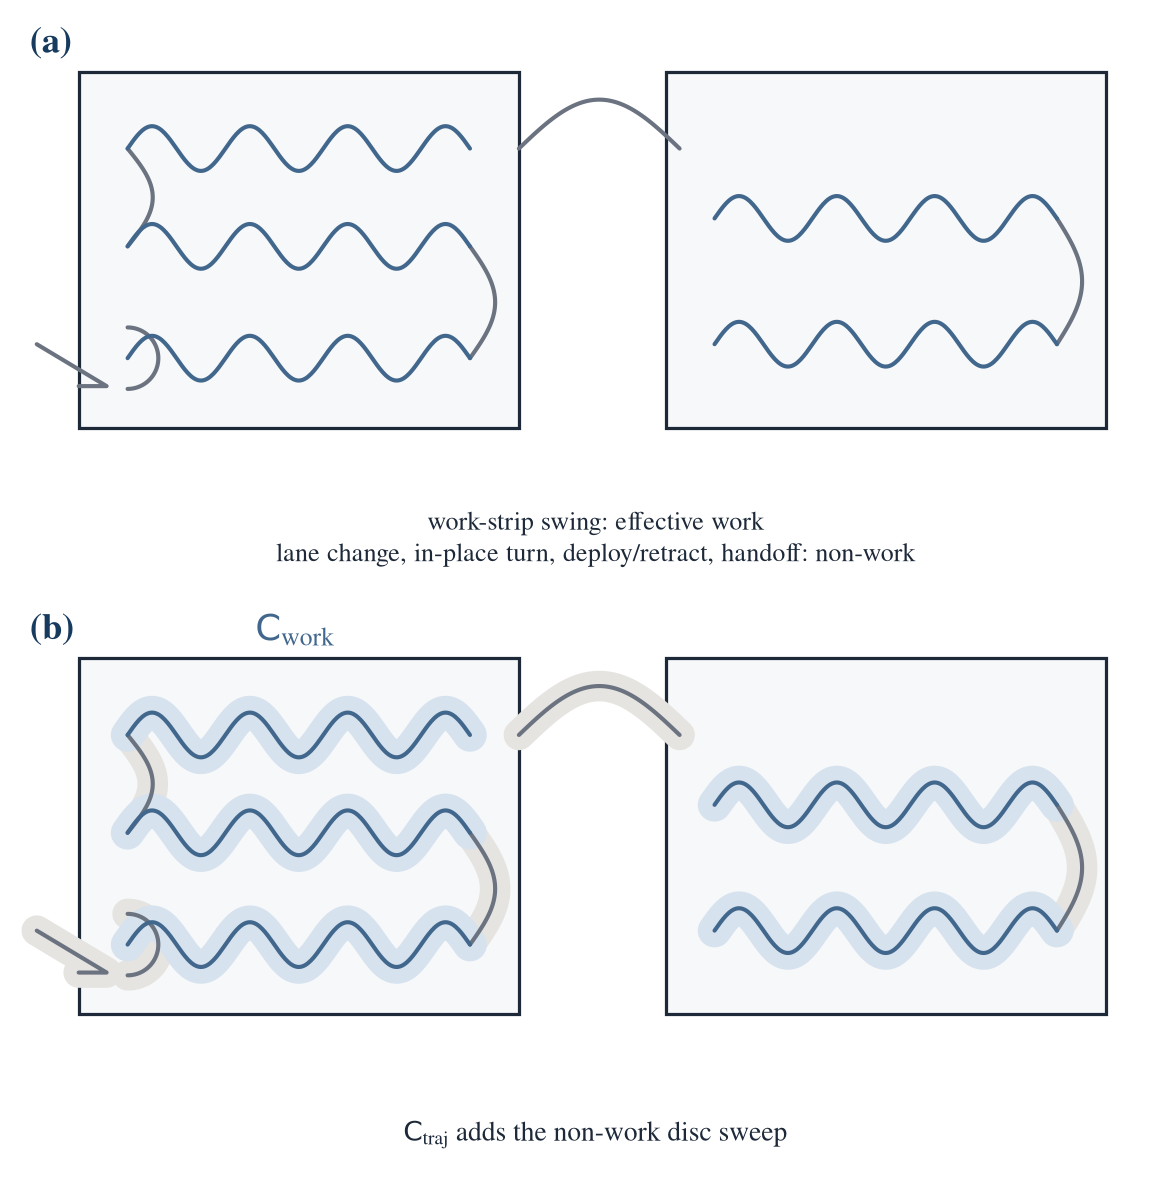
\includegraphics[width=0.92\linewidth]{figure_coverage_segments.png}
\end{figure}

For any segment $s$, let the disc-center path be
\begin{equation}
\mathbf p_d^s(\tau),\qquad \tau\in[0,T_s].
\tag{23}
\label{eq:segment-center}
\end{equation}
The disc-swept region of the segment is
\begin{equation}
\mathcal C_s=\bigcup_{\tau\in[0,T_s]}\left\{\mathbf z:\|\mathbf z-\mathbf p_d^s(\tau)\|_2\le r_d\right\}.
\tag{24}
\label{eq:segment-sweep}
\end{equation}

Let $\mathcal S_{\mathrm{work}}$ be the set of effective-work segments and $\mathcal S_{\mathrm{all}}$ the set of all motion segments. The method distinguishes
\begin{equation}
\mathcal C_{\mathrm{work}}=\bigcup_{s\in\mathcal S_{\mathrm{work}}}\mathcal C_s,
\qquad
\mathcal C_{\mathrm{traj}}=\bigcup_{s\in\mathcal S_{\mathrm{all}}}\mathcal C_s.
\tag{25}
\label{eq:work-and-trajectory-sweeps}
\end{equation}
The former contains only work-labeled disc sweeps, whereas the latter also includes disc motion during transfer, lane changes, and pose adjustment. Their respective coverage ratios are
\begin{equation}
\begin{aligned}
\rho_{\mathrm{work}}&=\frac{|\Pi_p(\mathcal C_{\mathrm{work}})\cap\mathcal P_F|}{|\mathcal P_F|},\\
\rho_{\mathrm{traj}}&=\frac{|\Pi_p(\mathcal C_{\mathrm{traj}})\cap\mathcal P_F|}{|\mathcal P_F|},
\end{aligned}
\tag{26}
\label{eq:coverage-ratios}
\end{equation}
where $\Pi_p(\cdot)$ rasterizes a continuous world-coordinate region into a pixel set. The primary coverage measure is $\rho_{\mathrm{work}}$ because it corresponds to explicitly labeled effective-work motion. The value $\rho_{\mathrm{traj}}$ describes how much free area is swept over the complete motion. If the disc remains in contact with the floor during non-working transfers, it captures additional physical sweeping; if the disc is lifted, it is only an auxiliary measure of path reach or potential sweep and must not be conflated with effective work coverage.

To avoid dependence on an arbitrary sampling frame rate, $\mathbf p_d^s(\tau)$ is recursively subdivided. A time interval $[\tau_a,\tau_b]$ is accepted only when the endpoint chord length is no greater than $\eta_\ell$ and the deviation of the midpoint from that chord is no greater than $\eta_c$. Both are chosen no larger than $s_p/2$, bounding discretization error by map resolution. Let the final subdivision points be $\mathbf c_0,\ldots,\mathbf c_m$. Rasterizing the radius-$r_d$ capsule between every adjacent pair yields
\begin{equation}
\widehat{\mathcal C}_s=\Pi_p\!\left(\bigcup_{j=0}^{m-1}\mathrm{Capsule}(\mathbf c_j,\mathbf c_{j+1},r_d)\right).
\tag{27}
\label{eq:rasterized-sweep}
\end{equation}
The capsule union is constructed in world coordinates before conversion by $\Pi_p$, avoiding a type mismatch between continuous regions and pixel sets. This method is more stable than drawing discs only at fixed-rate samples, especially during fast arm motion.

Finally, nominal execution time and planning time are
\begin{equation}
T_{\mathrm{exec}}=\sum_{s\in\mathcal S_{\mathrm{all}}}T_s,
\qquad
T_{\mathrm{plan}}=t_{\mathrm{eval,end}}-t_{\mathrm{raster,start}}.
\tag{28}
\label{eq:timing-measures}
\end{equation}
The first follows the piecewise-constant and serial-timing assumptions used for the local primitives. The second is measured as wall-clock time in one process, from conservative-grid generation through continuous-sweep evaluation. It includes decomposition, connectivity completion, route search, trajectory assembly, and coverage computation, but excludes map-file reading, output writing, and visualization. Thus $\rho_{\mathrm{work}}$, $\rho_{\mathrm{traj}}$, $T_{\mathrm{exec}}$, and $T_{\mathrm{plan}}$ match the output definitions in Fig.~\ref{fig:pipeline}.
